\section{旋转建模法}
所谓旋转建模法是通过绘制能够表征回转体特征的平面,然后用此平面绕其轴线旋转来一定角度来构建物体模型的方法。为便于叙述,我们将用于表征回转体特征的平面称之为特征平面,如图\ref{fig:tezhengpinmian.png}所示。图\ref{fig:xuanzhuanfa}所示的物体是用图\ref{fig:tezhengpinmian.png}所示的特征平面旋转$360^o$构建的。
\begin{figure}[htbp]
\subfloat[特征平面]{\label{fig:tezhengpinmian.png}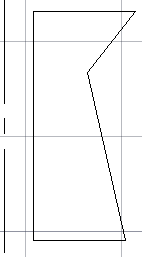
\includegraphics[scale=0.7]{tezhengpinmian.png}}\hspace{60pt}
\subfloat[回转体]{\label{fig:xuanzhuanfa}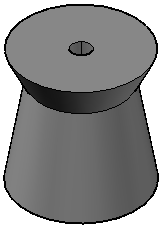
\includegraphics[scale=0.8]{xuanzhuanfa.png}}
\caption{旋转建模法}
\end{figure}
通过观察图\ref{fig:tiaoyafabei}所示杯零件图的左视图,我们可以得出其特征图为L型图形。
\subsection{绘制杯零件特征图}\label{sec:beilingjiantezheng}
在AutoCAD中,可以采取多种方法绘制杯零件特征图。下面我们以直接绘法、修剪法和集合法来实现杯零件特征图的绘制。
\subsubsection{直接绘制法}\label{sec:beilingjianleft}
所谓直接绘制法就是根据要绘制图形的图线构成,采用相应的AutoCAD命令完成图形绘制的方法。这种方法简单直观。图\ref{fig:tiaoyafabei}所示杯零件图的特征图均由直线构成,因而只需要用AutoCAD中的直线绘制命令即可完成。
\begin{procedure}

\item 启动AutoCAD软件。

启动AutoCAD软件的方法通常有:
\begin{itemize}
\item 双击桌面图标
\includegraphics[scale=0.2]{cadicon.png}。
\item 【开始】$\rightarrow$ 【所有程序】$\rightarrow$【Autodesk】$\rightarrow$【AutoCAD 2013 – 简体中文 (Simplified Chinese)】$\rightarrow$【AutoCAD 2013 – 简体中文 (Simplified Chinese)】。
\end{itemize}
AutoCAD软件启动完成后,将出现图\ref{fig:cadui}所示的软件界面。
\begin{figure}[htbp]
\centering
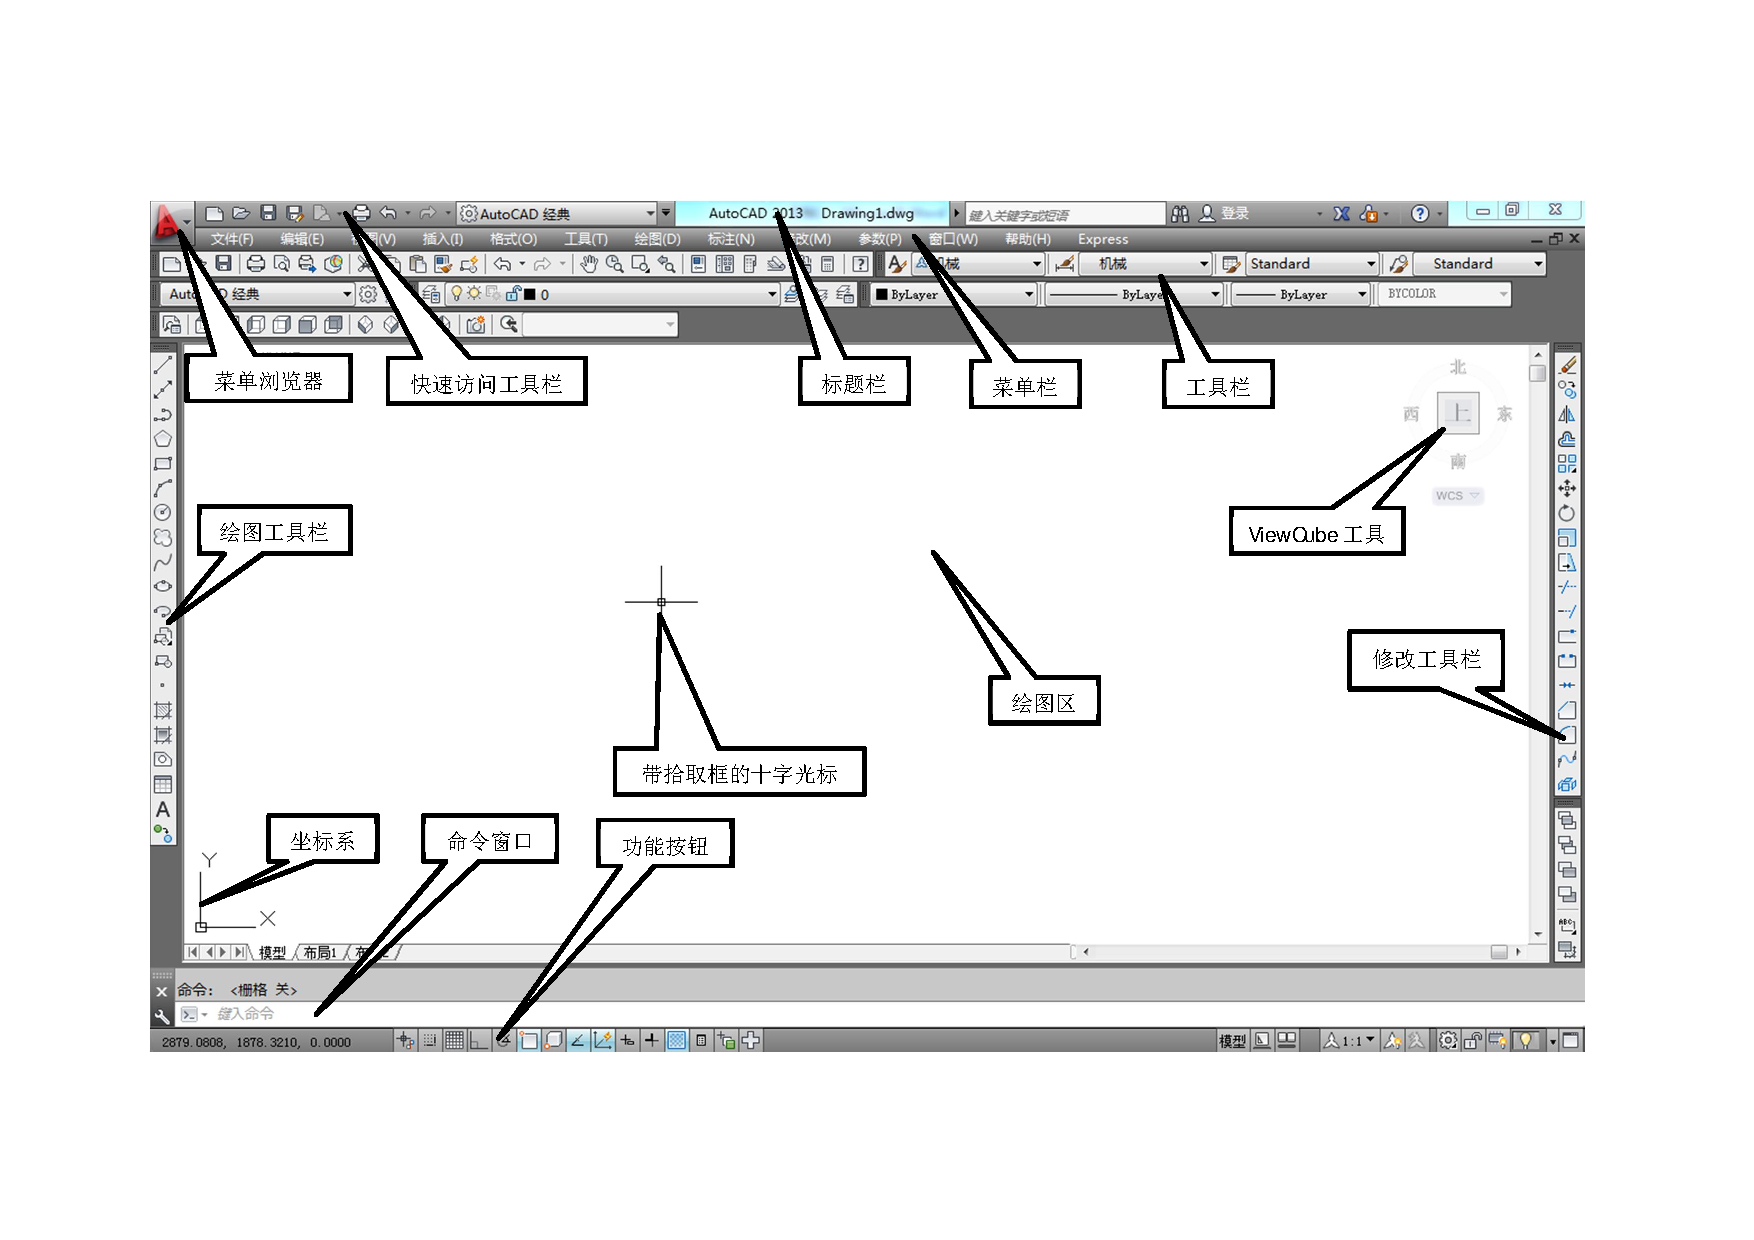
\includegraphics[scale=0.5]{cadui.pdf}
\caption{“AutoCAD经典”工作空间}\label{fig:cadui}
\end{figure}
AutoCAD软件的界面与Word字处理软件的界面非常相似,也是由标题栏、菜单栏、工具栏、绘图区、状态栏等要素构成。不同的是AutoCAD软件的界面在标题栏上还有菜单浏览器和快速访问工具栏;绘图区的左下方有坐标系,右上方有ViewCube工具,左边有绘图工具栏,右边有编辑工具栏;状态栏的上方有命令窗口;状态栏中有功能按钮。

\item 将视图切换为左视图。

AutoCAD启动后默认的视图方向是俯视图方向,而杯零件的特征图位于左视图方向,为了方便使用旋转法进行杯零件的三维建模,需要将AutoCAD的视图方向切换为左视图方向。实现左视图切换的方法有:
\begin{itemize}
\item 键盘输入-VIME\index{-view} 或-V,选择【正交】选项中的【左视】项。
\item 键盘输入-VIME,并输入left。
\item 【视图】$\rightarrow$【三维视图】$\rightarrow$【左视图】。
\item 【视图】$\triangleright$【左视】图标
\includegraphics[scale=0.6]{toptool.png}。
\end{itemize}
同理,如果要将视图切换为其它视图方向,其操作方法与切换左视图的方法是一致的,只是需要将“左视”换成其它视图方向即可。例如要将视图方向切换为俯视图方向则将上述方法中的【左视】改为【俯视】。

\item 启动【直线】命令

直线命令的启动方法有以下几种:
\begin{itemize}
\item 键盘输入line\index{line} 或L。
\item 【绘图】$\rightarrow$【直线】。
\item 【绘图】$\triangleright$【直线】图标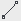
\includegraphics[scale=0.6]{linetool.png}。
\end{itemize}
在命令窗口中输入Line并按回车键或者空格键来启动命令。
\begin{lstlisting}
|命令: LINE|
|指定第一个点:
\end{lstlisting}
完成命令输入后,绘图区中的光标形状由带拾取框的十字光标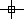
\includegraphics[scale=0.8]{guangbiao1} 变成十字形光标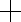
\includegraphics[scale=0.6]{guangbiao2}。
命令窗口中提示输入第一个点。在AutoCAD中每一个对象的点都是由具体的坐标进行表示的。因此在AutoCAD中可以通过以下三种方式输入点的坐标:
\begin{itemize}
\item 坐标数字
\item 光标直接输入
\item 光标捕捉方式输入
\end{itemize}

其中坐标数字和光标捕捉方式能够获得精确的坐标位置,因此能够实现图形的精确绘制,这也是AutoCAD软件绘图的特色之一。采用光标直接输入坐标非常不准确,误差很大,不能够实现图形的精确绘制。
\item 输入图线坐标点,实现封闭图形的绘制。

\begin{lstlisting}
|指定第一个点:0,0|
|指定下一点或 [放弃(U)]: 15$<$0|
|指定下一点或 [放弃(U)]: $@4<90$|
|指定下一点或 [闭合(C)/放弃(U)]: $@-10<0$|
|指定下一点或 [闭合(C)/放弃(U)]: $@11<90$|
|指定下一点或 [闭合(C)/放弃(U)]: $@-5<0$|
|指定下一点或 [闭合(C)/放弃(U)]: c|
\end{lstlisting}

至此,我们完成了杯零件的特征图绘制,结果如图\ref{fig:bettezheng}所示。
\noindent
\begin{figure}[htbp]
\centering
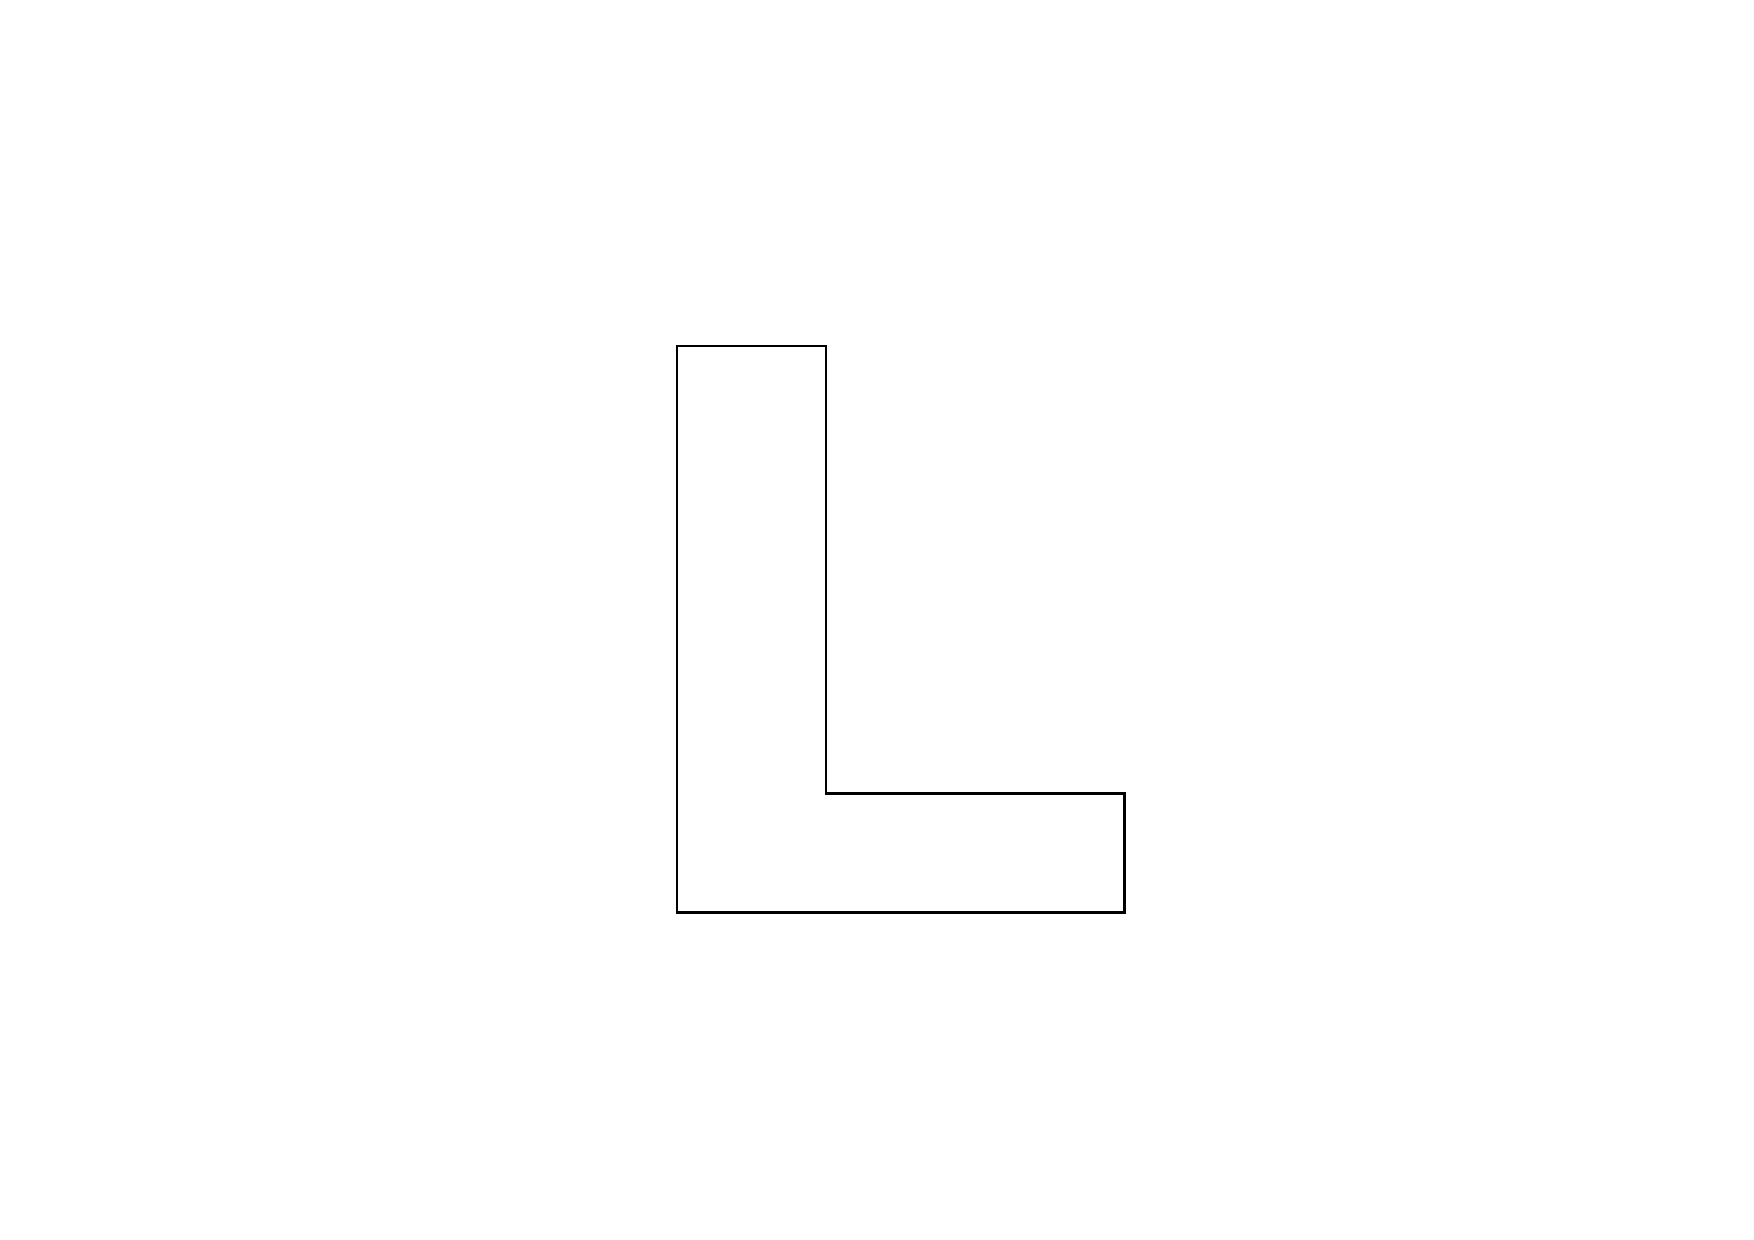
\includegraphics[scale=0.4]{beitezheng.pdf}
\caption{杯零件三维建模基础图}\label{fig:bettezheng}
\end{figure}
\end{procedure}

\subsubsection{坐标知识}
在第\ref{sec:beilingjianleft}节的操作中,我们用到了四种不同的坐标表达形式,它们分别是绝对直角坐标、相对直角坐标、绝对极轴坐标和相对极轴坐标。其中绝对直角坐表示与数学中的直角坐标表示是一致的,在AutoCAD中称为世界坐,其表示形式为$(x,y)$,图\ref{fig:zuobiao1}中$(0,0)$和$(2,1)$为绝对坐标表示。相对直角坐标表示则是将图形中的某一点假设为坐标原点,并以此为参照点来表示图形中的其它点,在AutoCAD中用$(@x,y)$的形式进行表示,图\ref{fig:zuobiao1}中的$(@2,1)$是以$(2,1)$为参照坐标原点$(0',0')$进行表示的,其值分别是相对于参照原点的$x$和$y$坐标增量。绝对极轴坐标表示是用点与点之间的线段长度以及该连线与水平线之间的夹角来表示点的具体位置,在AutoCAD中用$(@$距离$<$角度$)$的形式表示,图\ref{fig:jizuobiao1}中的$(0<0\degree)$为极轴坐标的原点表示,$(1<45\degree)$为点在绝对极轴坐标中的位置表示。相对极轴坐标表示与相对直角坐标表示类似,也是以将图形中的某一点作为参照极轴坐标原点,并以此为参照来表示图形中其它点的位置。绝对直角坐标和绝对极轴坐标表示都要求准确地给出物体每一个点在AutoCAD世界坐标系中的准确位置,对于简单的图形是可行的,对于复杂的图形,会存在计算比较大,不能够满足快速绘图需要的缺点。相对直角坐标和相对极轴坐标表示是用增量进行表示,因此计算简单、直观,较好地满足了快速绘图的需要。实际应用中,需要根据图形的特点来选择适当的坐标表示法。总之,坐标表示方式的选择原则是:以方便表示,减少计算量为目标。
\begin{figure}[htbp]
\centering
\begin{floatrow}
\ffigbox{\caption{直角坐标表示}\label{fig:zuobiao1}}{
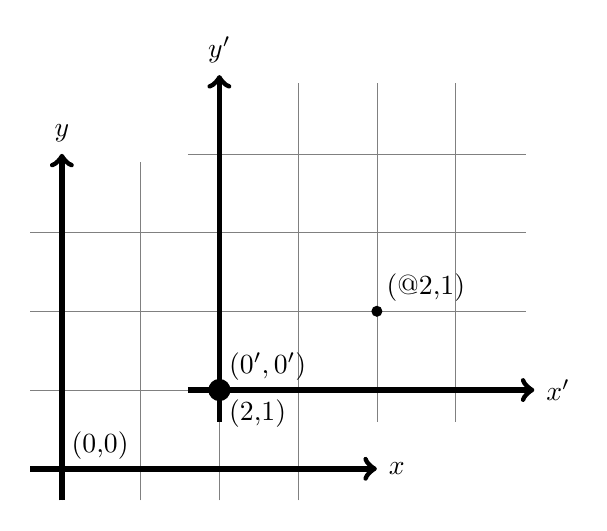
\begin{tikzpicture}
\draw[help lines,step=1cm,very thin](-0.4cm,-0.4cm)grid(3.9cm,3.9cm);
\draw[->,line width=0.7mm](-0.4cm,0)--(4cm,0)node[right]{$x$};
\draw[->,line width=0.7mm](0,-0.4cm)--(0,4cm)node[above]{$y$};
\draw (0,0)node[above right]{(0,0)};
\fill (2cm,1cm)node[below right]{(2,1)}circle(4pt);
\begin{scope}[shift={(2cm,1cm)}]
\draw[help lines,step=1cm,very thin](-0.4cm,-0.4cm)grid(3.9cm,3.9cm);
\draw[->,line width=0.7mm](-0.4cm,0)--(4cm,0)node[right]{$x'$};
\draw[->,line width=0.7mm](0,-0.4cm)--(0,4cm)node[above]{$y'$};
\draw (0,0)node[above right]{$(0',0')$};
\fill (2cm,1cm)node[above right]{(@2,1)}circle(2pt);
\end{scope}
\end{tikzpicture}}
\ffigbox{\caption{极轴坐标表示}\label{fig:jizuobiao1}}{
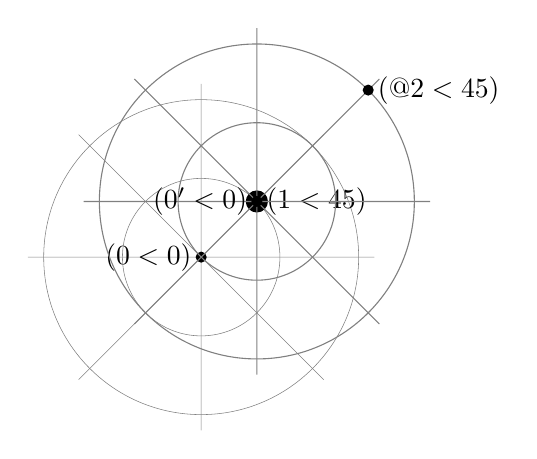
\begin{tikzpicture}
\draw[help lines,very thin](-2.2cm,0)--(2.2cm,0)(0,-2.2cm)--(0,2.2cm)(45:2.2cm)--(225:2.2cm)(135:2.2cm)--(-45:2.2cm);
\fill(0,0)node[left]{($0<0\degree$)}circle(2pt);
\draw[help lines,very thin](0,0)circle(1cm)circle(2cm);
\fill (45:1cm)node[above,right]{$(1<45\degree)$}circle(4pt);
\begin{scope}[shift={(45:1cm)}]
\draw[help lines,thin](-2.2cm,0)--(2.2cm,0)(0,-2.2cm)--(0,2.2cm)(45:2.2cm)--(225:2.2cm)(135:2.2cm)--(-45:2.2cm);
\draw[help lines,thin](0,0)circle(1cm)circle(2cm);
\fill (45:2cm)node[right]{$(@2<45\degree)$}circle(2pt);
\fill(0,0)node[below,left]{($0'<0\degree$)}circle(2pt);
\end{scope}
\end{tikzpicture}
}
\end{floatrow}
\end{figure}
直线命令的注意事项和技巧:

\begin{tips}
\item 输入坐标点时,坐标数字和逗号必须是半角状态的数字和逗号。如果为全角状态将出现错误。
\item 在使用Line命令的过程中,如果由于输入坐标错误或误点鼠标而导线段绘制错误,在没有结束命令的前提下,可以直接输入U来撤消上一次绘制的线段。
\item 在使用Line命令过程中,如果还没有完成图形的绘制就提前结束了命令,可以再次使用直线命令,并利用端点捕捉的方式获得命令结束时所绘制端点的坐标,然后接着完成图形的绘制。开启端点捕捉的方法有:
\begin{itemize}
\item 绘图过程中用键盘输入:end。
\item 绘图过程中按ctrl或shift键+鼠标右击弹出图\ref{fig:duixiangbuzuomen2}所示的【对象捕捉】菜单,并选择【端点】项。
\begin{figure}[htbp]
\centering
\begin{floatrow}
\ffigbox[2.2\FBwidth]{\caption{“对象捕捉”菜单一}\label{fig:duixiangbuzuomen2}}{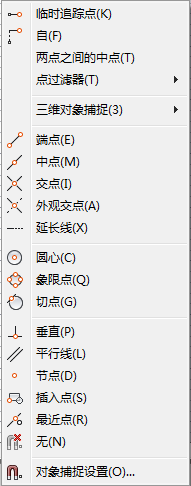
\includegraphics[scale=0.5]{duixiangbuzuomen2.png}}
\ffigbox[2.2\FBwidth]{\caption{“对象捕捉”菜单二}\label{fig:duixiangbuzuomen1}}{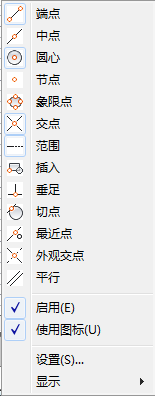
\includegraphics[scale=0.6]{duixiangbuzuomen1.png}}
\end{floatrow}
\end{figure}
\item 在功能按钮区中将对象捕捉图标由
\includegraphics[scale=0.6]{duixiangbuzuo1.png}状态设置为
\includegraphics[scale=0.6]{duixiangbuzuo.png}状态,并在图标上右击弹出图\ref{fig:duixiangbuzuomen1}所示的【对象捕捉】菜单,并使【端点】项为开启状态。
\end{itemize}
\item 直线命令的C选项用于将最后一点与第一点连接起来并结束命令。
\item 使用坐标和捕捉是实现AutoCAD精确绘图的关键。
\end{tips}



\subsubsection{修剪法}
所谓修剪法是先通过绘制一些简单的基础图形,然后经过简单的编辑和修改的方式来获得图形的方法,亦可称之为编辑法。本节我们将用修剪法来完成图\ref{fig:bettezheng}的绘制。
\begin{procedure}
\item 绘制两条相互垂直的直线,作为基础。
\begin{lstlisting}
|命令: LINE|
|指定第一个点:0,15|
|指定下一点或 [放弃(U)]: @0,-15|
|指定下一点或 [放弃(U)]: $@15<0$|
|指定下一点或 [闭合(C)/放弃(U)]: |
\end{lstlisting}
\item 用偏移产生符合尺寸距离的水平线。启动【偏移】命令的方法有:
\begin{itemize}
\item 键盘输入OFFSET\index{offset}或O。
\item 【修改】$\rightarrow$【偏移】。
\item 【修改】$\triangleright$【偏移】图标
\includegraphics[scale=0.6]{offsettool.png}。
\end{itemize}
启动【偏移】命令后,AutoCAD要求指定图形的偏移距离。
\begin{lstlisting}
|命令:OFFSET|
|当前设置: 删除源=否  图层=源  OFFSETGAPTYPE=0|
|指定偏移距离或 [通过(T)/删除(E)/图层(L)] $<$通过$>$:  4|
\end{lstlisting}
指定偏移距离后,要求选择用于偏移的对象,此时用鼠标选择图\ref{fig:trimmotherd}中的水平线,选中后该水平线将以虚线形式表示,如图\ref{fig:offsetselect}所示。
\begin{lstlisting}
|选择要偏移的对象,或 [退出(E)/放弃(U)] $<$退出$>$:|
\end{lstlisting}
接下来,要求指定图形向哪一侧偏移,此时将鼠标移至选中水平线的上方,并单击鼠标左键,即完成一次图形的偏移操作。
\begin{lstlisting}
|指定要偏移的那一侧上的点,或[退出(E)/多个(M)/放弃(U)]|
|$<$退出$>$:|
|选择要偏移的对象,或 [退出(E)/放弃(U)] $<$退出$>$:|
\end{lstlisting}
然后,再用相同的方法得到另一条水平线。
\begin{lstlisting}
|命令: OFFSET|
|当前设置: 删除源=否  图层=源  OFFSETGAPTYPE=0|
|指定偏移距离或 [通过(T)/删除(E)/图层(L)] $<4.0000>$:  11|
|选择要偏移的对象,或 [退出(E)/放弃(U)] $<$退出$>$:|
|指定要偏移的那一侧上的点,或 [退出(E)/多个(M)/放弃(U)] |
|$<$退出$>$:|
|选择要偏移的对象,或 [退出(E)/放弃(U)] $<$退出$>$:|
\end{lstlisting}

\item 用偏移产生符合尺寸距离的垂直线。
\begin{lstlisting}
|命令:OFFSET|
|当前设置: 删除源=否  图层=源  OFFSETGAPTYPE=0|
|指定偏移距离或 [通过(T)/删除(E)/图层(L)] $<11.0000>$:  5|
|选择要偏移的对象,或 [退出(E)/放弃(U)] $<$退出$>$:|
|指定要偏移的那一侧上的点,或[退出(E)/多个(M)/放弃(U)]|
|$<$退出$>$:|
|选择要偏移的对象,或 [退出(E)/放弃(U)] $<$退出$>$:|
|命令: OFFSET|
|当前设置: 删除源=否  图层=源  OFFSETGAPTYPE=0|
|指定偏移距离或 [通过(T)/删除(E)/图层(L)] $<5.0000>$:  10|
|选择要偏移的对象,或 [退出(E)/放弃(U)] $<$退出$>$:|
|指定要偏移的那一侧上的点,或 [退出(E)/多个(M)/放弃(U)] |
|$<$退出$>$:|
|选择要偏移的对象,或 [退出(E)/放弃(U)] $<$退出$>$:|
\end{lstlisting}
\begin{figure}[htbp]
\centering
\subfloat[]{\label{fig:trimmotherd}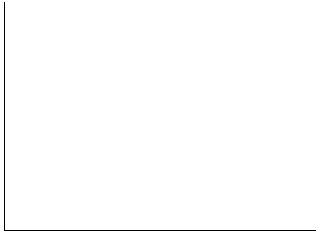
\includegraphics[scale=0.4]{trimmotherd1.png}}\hspace{20pt}
\subfloat[]{\label{fig:offsetselect}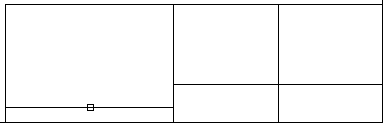
\includegraphics[scale=0.4]{offsetselect.png}}\hspace{20pt}
\subfloat[]{\label{fig:offsetresult}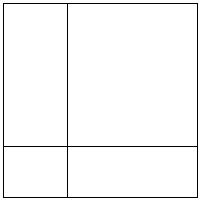
\includegraphics[scale=0.5]{offsetresult.png}}
\caption{偏移过程}
\end{figure}
\item 修剪图形。

图\ref{fig:offsetresult}为完成偏移操作后的结果,需要用【修剪】命令修剪掉多余的线段,以获得最终图形。【修剪】命令的启动方法有:
\begin{itemize}
\item 解盘输入TRIM\index{trim} 或TR。
\item 【修改】$\rightarrow$【修剪】。
\item 【修改】$\triangleright$【修剪】图标
\includegraphics[scale=0.6]{trimtool.png}。
\end{itemize}
启动修剪命令后要求指定用于修剪的边,其命令提示为:
\begin{lstlisting}
|命令: TRIM|
|当前设置:投影=UCS,边=无|
|选择剪切边...|
\end{lstlisting}
此时,用框选方式选择所有的图线用作剪切边,选择方法如图\ref{fig:trimegeselect}所示,选择结果如图\ref{fig:trimselectresult}所示。其命令提示为:
\begin{lstlisting}
|选择对象或 $<$全部选择$>$:  指定对角点: 找到 6 个|
|选择对象:|
\end{lstlisting}
结束修剪边的选择后,要求选择要修剪的线段或者对象。同样用框选方式选择要修剪的对象,选择方法如图\ref{fig:trimedselect}所示,修剪完成后,其结果如图\ref{fig:trimedresult}所示。其命令提示为:
\begin{lstlisting}
|选择要修剪的对象,或按住 Shift 键选择要延伸的对象,或|
|[栏选(F)/窗交(C)/投影(P)/边(E)/删除(R)/放弃(U)]:  指定对角点:|
\end{lstlisting}
再用拾取的方式将剩下的多余的线段修剪掉,得到图\ref{fig:bettezheng}所示的图形。其命令提示为:
\begin{lstlisting}
|选择要修剪的对象,或按住 Shift 键选择要延伸的对象,或|
|[栏选(F)/窗交(C)/投影(P)/边(E)/删除(R)/放弃(U)]:|
|选择要修剪的对象,或按住 Shift 键选择要延伸的对象,或|
|[栏选(F)/窗交(C)/投影(P)/边(E)/删除(R)/放弃(U)]:|
|选择要修剪的对象,或按住 Shift 键选择要延伸的对象,或|
|[栏选(F)/窗交(C)/投影(P)/边(E)/删除(R)/放弃(U)]:|
\end{lstlisting}
\begin{figure}[htbp]
\centering
\subfloat[]{\label{fig:trimegeselect}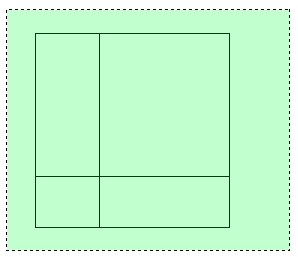
\includegraphics[scale=0.3]{trimegeselect.png}}\hspace{20pt}
\subfloat[]{\label{fig:trimselectresult}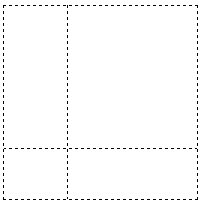
\includegraphics[scale=0.3]{trimselectresult.png}}\hspace{20pt}
\subfloat[]{\label{fig:trimedselect}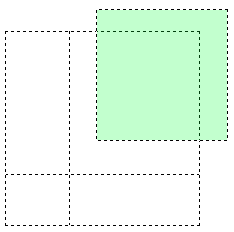
\includegraphics[scale=0.3]{trimedselect.png}}\hspace{20pt}
\subfloat[]{\label{fig:trimedresult}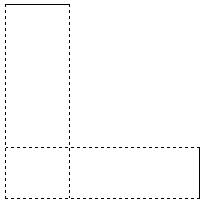
\includegraphics[scale=0.3]{trimedresult.png}}
\caption{修剪过程}
\end{figure}
\end{procedure}

偏移命令和修剪命令的注意事项和技巧:
\begin{tips}
\item 【偏移】操作过程中,如果多次偏移的距离相同则可以多次选择对象并执行偏移。
\item 【修剪】操作的关键是修剪边的选择,若要剪去某线段之外的图线,则应选择该线段作为修剪边;若要剪去某两条线段之间的图线则要选择该两条线段,否则不能够实现操作目的。
\item 【修剪】操作中修剪对象的选择具有一定的顺序,一般为先剪去外围不需要的图线,再剪去内部的图线,否会出现部分图线不能够剪除,只能够删除的现象。
\end{tips}

\subsubsection{集合法}
所谓集合法就是通过绘制简单的封闭图形(如矩形、圆);然后将利用这些封闭图形生成面域;最后利用简单图形面域之间的并集、差集和交集关系来获得图形的方法。所谓面域是具有物理特性(例如,质心)的二维封闭区域。图\ref{fig:bettezheng}所示的杯零件特征图能够看作是用一个大的矩形面域减去一个小的矩形面域。
\begin{procedure}
\item 绘制大矩形。

启动绘制矩形命令的方法有:
\begin{itemize}
\item 键盘输入RECTANGLE\index{rectangle}或REC
\item 【绘图】$\rightarrow$【矩形】。
\item 【绘图】$\triangleright$【矩形】图标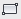
\includegraphics[scale=0.6]{rectangletool.png}
\end{itemize}
\begin{lstlisting}
|命令: rectang|
|指定第一个角点或 [倒角(C)/标高(E)/圆角(F)/厚度(T)/宽度(W)]: 0,0|
|指定另一个角点或 [面积(A)/尺寸(D)/旋转(R)]: @15,15|
\end{lstlisting}
\item 绘制小矩形,结果如图\ref{fig:bei1}所示。
\begin{lstlisting}
|命令: rectang|
|指定第一个角点或 [倒角(C)/标高(E)/圆角(F)/厚度(T)|
|/宽度(W)]:15,15|
|指定另一个角点或 [面积(A)/尺寸(D)/旋转(R)]: @-10,-11|
\end{lstlisting}
\item 面域矩形矩形。

启动【面域】命令的方法有:
\begin{itemize}
\item 解盘输入REGION\index{region}或REG。
\item 【绘图】$\rightarrow$【面域】。
\item 【绘图】$\triangleright$【面域】图标
\includegraphics[scale=0.6]{regiontool.png}。
\end{itemize}
以框选的方式选择两个要面域的矩形,选中后两个矩形均以虚线的形式表示,结果如图\ref{fig:bei2}所示。
\begin{lstlisting}
|命令:REGION|
|选择对象: 指定对角点: 找到 2 个|
|选择对象:|
|已提取 2 个环。|
|已创建 2 个面域。|
\end{lstlisting}
正确执行面域命令后,AutoCAD会提示该命令提取了几个封闭环,创建了几个面域。
\begin{figure}[htbp]
\centering
\subfloat[绘制矩形结果]{\label{fig:bei1}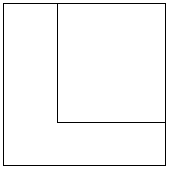
\includegraphics[scale=0.7]{bei1.png}}\hspace{20pt}
\subfloat[面域选择]{\label{fig:bei2}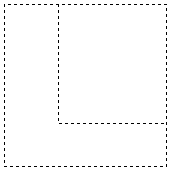
\includegraphics[scale=0.7]{bei2.png}}\hspace{20pt}
\subfloat[选择被减对象]{\label{fig:bei3}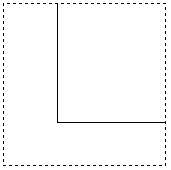
\includegraphics[scale=0.7]{bei3.png}}\\
\subfloat[选择减对象]{\label{fig:bei4}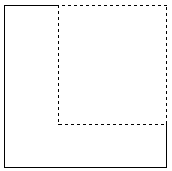
\includegraphics[scale=0.7]{bei4.png}}\hspace{20pt}
\subfloat[差集结果]{\label{fig:bei5}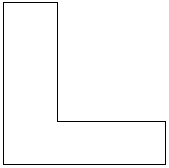
\includegraphics[scale=0.7]{bei5.png}}
\caption{集合法}
\end{figure}
\item 进行差集操作。

要实现从大矩形中减去小矩形,需要用到实体编辑中的【差集】命令,其启动方法有:
\begin{itemize}
\item 键盘输入SUBTRACT\index{subtract}或SU。
\item 【修改】$\rightarrow$【实体编辑】$\rightarrow$【差集】。
\item 【实体编辑】$\triangleright$【差集】图标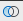
\includegraphics[scale=0.7]{subtracttool.png}。
\end{itemize}
选择大矩形作为被减对象,被选中的矩形以虚线形式表示,结果如图\ref{fig:bei3}所示。
\begin{lstlisting}
|命令: SUBTRACT|
|选择要从中减去的实体、曲面和面域...|
|选择对象: 找到 1 个|
\end{lstlisting}
选择小矩形作为减去对象,被选中的矩形以虚线形式表示,结果如图\ref{fig:bei4}所示。
\begin{lstlisting}
|选择对象:  选择要减去的实体、曲面和面域...|
|选择对象: 找到 1 个|
|选择对象:|
\end{lstlisting}
图\ref{fig:bei5}为差集操作后的结果,也图\ref{fig:bettezheng}的结果是一致的。由此可见在AutoCAD中完成同样的图形绘制可能采取不同的方法和策略。

\end{procedure}

集合法绘制图形的注意事项和技巧:
\begin{tips}
\item 用于集合运算的对象必须是面域对象或者实体。
\item 尽管矩形、圆、正多边是封闭线框,但不是面域对象,因此需要先进行面域操作后,才能够进行并、差、交等集合操作。
\end{tips}
\endinput